%%%%%%%%%%%%%%%%%%%%%%%%%%%%%%%%%%%%%%%%%
% Beamer Presentation
% LaTeX Template
% Version 1.0 (10/11/12)
%
% This template has been downloaded from:
% http://www.LaTeXTemplates.com
%
% License:
% CC BY-NC-SA 3.0 (http://creativecommons.org/licenses/by-nc-sa/3.0/)
%
%%%%%%%%%%%%%%%%%%%%%%%%%%%%%%%%%%%%%%%%%
%
% Math 370 (Mathematical Modeling), Fall 2014
% Semester Project: Final Presentation
% (C) 2014 Peter Gordon <peter.gordon@csu.fullerton.edu>,
%	Casey Cao-Son <dangkhoa27@gmail.com>,
%	Brennan Truong <brennantruong@gmail.com>
%
%%%%%%%%%%%%%%%%%%%%%%%%%%%%%%%%%%%%%%%%%
%----------------------------------------------------------------------------------------
%	PACKAGES AND THEMES
%----------------------------------------------------------------------------------------

\documentclass{beamer}

\mode<presentation> {

% The Beamer class comes with a number of default slide themes
% which change the colors and layouts of slides. Below this is a list
% of all the themes, uncomment each in turn to see what they look like.

%\usetheme{default}
%\usetheme{AnnArbor}
%\usetheme{Antibes}
%\usetheme{Bergen}
%\usetheme{Berkeley}
%\usetheme{Berlin}
%\usetheme{Boadilla}
%\usetheme{CambridgeUS}
%\usetheme{Copenhagen}
%\usetheme{Darmstadt}
%\usetheme{Dresden}
%\usetheme{Frankfurt}
%\usetheme{Goettingen}
%\usetheme{Hannover}
%\usetheme{Ilmenau}
%\usetheme{JuanLesPins}
%\usetheme{Luebeck}
%\usetheme{Madrid}
%\usetheme{Malmoe}
%\usetheme{Marburg}
%\usetheme{Montpellier}
%\usetheme{PaloAlto}
%\usetheme{Pittsburgh}
%\usetheme{Rochester}
%\usetheme{Singapore}
%\usetheme{Szeged}
\usetheme{Warsaw}

% As well as themes, the Beamer class has a number of color themes
% for any slide theme. Uncomment each of these in turn to see how it
% changes the colors of your current slide theme.

%\usecolortheme{albatross}
%\usecolortheme{beaver}
%\usecolortheme{beetle}
%\usecolortheme{crane}
%\usecolortheme{dolphin}
%\usecolortheme{dove}
%\usecolortheme{fly}
%\usecolortheme{lily}
%\usecolortheme{orchid}
%\usecolortheme{rose}
%\usecolortheme{seagull}
%\usecolortheme{seahorse}
%\usecolortheme{whale}
%\usecolortheme{wolverine}

%setbeamertemplate{footline} % To remove the footer line in all slides uncomment this line
%setbeamertemplate{footline}[page number] % To replace the footer line in all slides with a simple slide count uncomment this line
%setbeamertemplate{footline}[frame number]
%setbeamertemplate{navigation symbols}{} % To remove the navigation symbols from the bottom of all slides uncomment this line
}

\usepackage{graphicx} % Allows including images
\usepackage{booktabs} % Allows the use of \toprule, \midrule and \bottomrule in tables
\usepackage{amsmath}
\usepackage{amsfonts}
\usepackage{amssymb}
\usepackage{amsthm}
\usepackage{float}
\usepackage{mathtools}

\DeclarePairedDelimiter{\abs}{\lvert}{\rvert}

%----------------------------------------------------------------------------------------
%	TITLE PAGE
%----------------------------------------------------------------------------------------
\title[The Minimum Steiner Tree Problem]{(1991) The Minimum Steiner Tree Problem}

\author{Peter Gordon, Casey Cao-Son, \& Brennan Truong}
% Your name
\institute[CSUF] % Your institution as it will appear on the bottom of every slide, may be shorthand to save space
{
California State University, Fullerton \\ % Your institution for the title page
\medskip
Mathematical Modeling, Semester Project \\
\medskip
\textit{peter.gordon@csu.fullerton.edu} \\ 
\textit{dangkhoa27@csu.fullerton.edu} \\
\textit{brennantruong@gmail.com} % Your email address
}
\date{Dec. 10, 2014} % Date, can be changed to a custom date

\begin{document}

\section{Introduction}
\begin{frame}
\titlepage % Print the title page as the first slide

\end{frame}


%begin{frame}
%frametitle{Table of Contents} % Table of contents slide, comment this block out to remove it
%tableofcontents % Throughout your presentation, if you choose to use \section{} and \subsection{} commands, these will automatically be printed on this slide as an overview of your presentation
%end{frame}

\subsection{Goal}
\begin{frame}
\frametitle{Introduction / Goal}
\begin{itemize}
\item<1-> {
	Modern communication is based on wired networks.
}

\item<2-> {
	Devices are connected through cables to transmit information.
}
\item<3-> {
	Total cost of network proportional to amount of cabling used:
	\[
		\text{Cost} \propto \sum_{i \in \{\text{cables}\}} {\text{Length}_i}
	\]
}

\item<4-> {
	Propagation delay (\(\frac{d}{s}\)) is also proportional to total amount of cabling:
	\[
		\frac{d}{s} \propto \sum_{i \in \{\text{cables}\}} {\text{Length}_i}
	\]
}
\item<5-> {
	\textbf{Goal:} Minimize cost and delay by reducing amount of cabling.
}
\end{itemize}
\end{frame}

\subsection{Definitions}
\begin{frame}
\frametitle{Definition: Weighted Graph / Adjacency}
\begin{block}{Weighted Graph}
\begin{itemize}
\item<1-> {
A \emph{weighted graph} \(G = (V, E)\) is a pair of a set of 
points (called \emph{vertices}) \(V\) and the set of \emph{edges}, \(E\), where each edge in \(E\) is a 3-tuple consisting of two 
vertices in \(V\) combined with a nonnegative real number \emph{weight}. \\ That is, each edge is an element of the form \((v_a, v_b, 
w_{a,b})\) with \(v_a\), \(v_b \in V\) and \(w_{a,b} \in \left\{x \in \mathbb{R} \,\vert\, x > 0\right\}\).
}
\item<2-> {
The \emph{weight of \(G\)} is the sum of all its edge weights.
} 
\end{itemize}
\end{block}
\begin{block}<3->{Adjacent Vertices}
\begin{itemize}
\item<3-> {
Given a weighted graph \(G\) = (\(V\), \(E\)), two vertices \(v_1\) and \(v_2\) in \(V\) are \emph{adjacent} provided that there exists an edge between them. 
}
\end{itemize}
\end{block}
\end{frame}

\begin{frame}
\frametitle{Definition: Connectedness / Vertex Order}
\begin{block}<1->{Connected Vertices}
\footnotesize\begin{itemize}
\item<1-> {
Any two vertices \(v_a\) and \(v_b\) are \emph{connected} provided that there exists an ordered sequence \(P\) of 
vertices \((v_{P_0} = v_a , v_{P_1}, v_{P_2}, \ldots, v_{P_{n-1}}, v_{P_n} = v_b)\) such that every sequential pair of vertices is 
adjacent. That is, \(v_a\) is adjacent to \(v_{P_1}\), \(v_{P_1}\) is adjacent to \(v_{P_2}\), and so on. 
}
\item<2-> {
\(P\) is called the 
\emph{path between} \(v_a\) and \(v_b\) (or alternatively, \(v_a\) and \(v_b\) are \emph{connected through} \(P\)).
}
\item<3-> {
A graph \(G\) is a \emph{connected graph} when all possible pairs of vertices are connected.
}
\end{itemize}
\end{block}
\begin{block}<4->{Vertex Order}
\small{ Given a weighted graph \(G = (V, E)\), The \emph{order (degree) of a vertex} \(v\) is the number of edges which connect \(v\) to another vertex in \(G\). }
\end{block}
\end{frame}


\begin{frame}
\frametitle{Definition: MST / Rectilinear Distance}
\begin{block}<1->{Minimum Spanning Tree}
\begin{itemize}
\item<1-> {
Given a connected graph \(G = (E, V)\), the \emph{spanning tree} \(T\) of \(G\) is a connected graph with the same vertices as \(G\), whose edges form a subset of \(E\), and in which each pair of vertices is connected through exactly one path.
}
\item<2-> {
\(T\) is the \emph{minimum spanning tree} of \(G\) provided that the weight of \(T\) is the smallest among all
spanning trees of \(G\).
}
\end{itemize}	
\end{block}

\begin{block}<3->{Rectilinear Distance}
The \emph{rectilinear distance}, \(d_1\),  between two points is the sum of the absolute values of the difference of their like coordinates.
\[d_1 (p, q) = \left|p_x - q_x\right| + \left|p_y - q_y\right|\]
\end{block}
\end{frame}

\subsection{Problem Statement}
\begin{frame}
\frametitle{Problem Statement}
\begin{block}<1->{The General Minimum Rectilinear Steiner Tree Problem}
(\#3) Given a set of Cartesian points \(S = \left\{p_1, p_2, \ldots, p_n\right\}\), find the minimum
spanning tree, using rectilinear distances, which connects all points in \(S\) using only horizontal
and vertical line segments, adding any intermediary points as needed.

\end{block}
\begin{block}<2->{Specific Data}
(\#1) Find the minimal-cost rectilinear spanning tree for a network with the following nine stations:
\[a(0, 15), \quad b(5, 20), \quad c(16, 24), \quad d(20, 20), \quad e(33, 25) \] \[ f(23, 11), \quad 
g(35, 7), \quad h(25, 0), \quad i(10, 3) \quad \text{.}\]
\end{block}
\end{frame}


\begin{frame}
\frametitle{Problem Statement}
\begin{block}<1->{Weighted Stations}
(\#2) Find a minimal-cost rectilinear spanning tree for the above network, but where each station adds a
weight of \(d^{3/2}w\), where \(w = 1.2\) and \(d\) is the degree of the vertex.
\end{block}
\begin{block}<2->{Method to Our Madness}
\begin{itemize}
\item<2-> {Questions answered out of their given order?}
\item<3-> {Creating a general solution first makes the other two "plug-and-chug"!}
\end{itemize}
\end{block}
\end{frame}

\section{Literature Review}
\subsection{Hanan's Theorem}
\begin{frame}
\frametitle{Hanan's Theorem}
\begin{block}<1->{Hanan Grid}
\noindent\begin{minipage}{0.4\textwidth}
Given a set of points, its \emph{Hanan Grid} is a grid composed of horizontal and vertical lines that intersect at all of the points.
\end{minipage}
\hfill
\begin{minipage}{0.45\textwidth}
\onslide<2-> \begin{figure}[Hp!]
	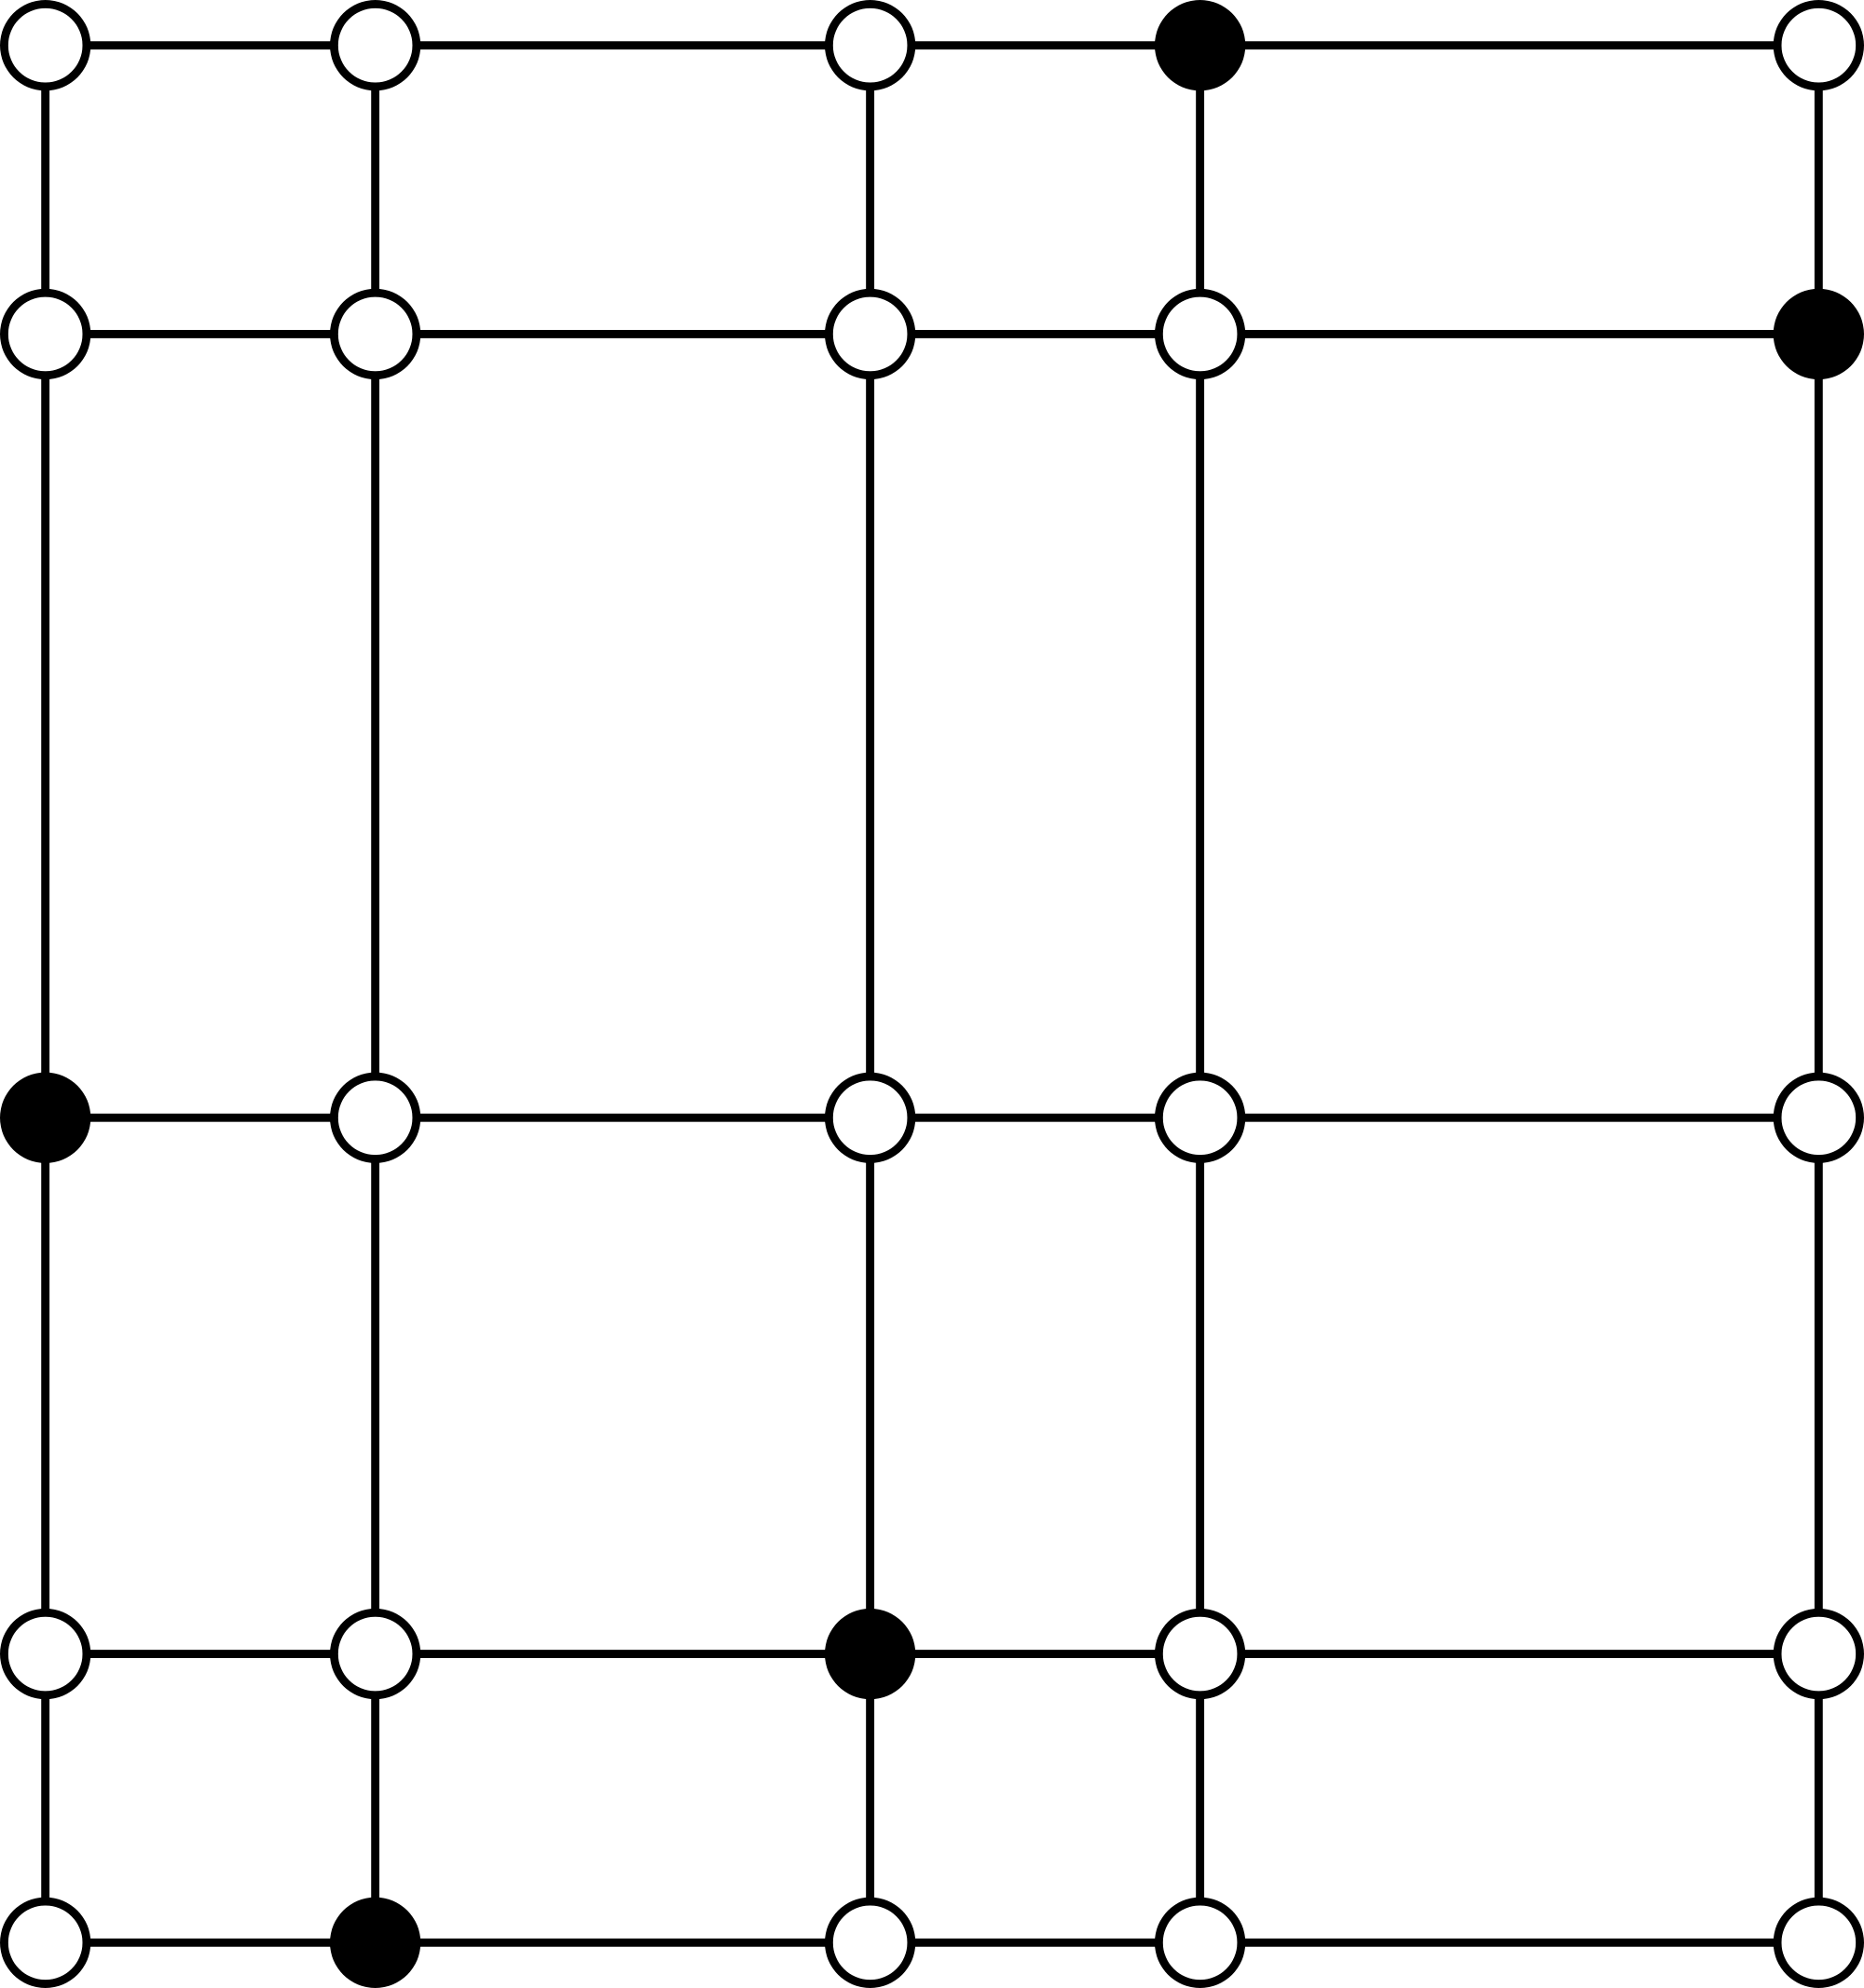
\includegraphics[width=0.4\textwidth]{HananGrid}
	\caption{Hanan grid generated for 5 points, by Jeffrey Sharkey, on Wikipedia.}
	\label{hanangrid_image}
\end{figure}
\end{minipage}
\end{block}
\begin{block}<3->{Hanan's Theorem}
\frametitle{Hanan's Theorem}
In 1966, Maurice Hanan proved: any MRST of a set of points \emph{must} have vertices on its Hanan grid.
\end{block}
\end{frame}

\begin{frame}
\frametitle{Manual MRST Construction via Hanan Grid}
\onslide<1-> \begin{figure}[Hp!]
	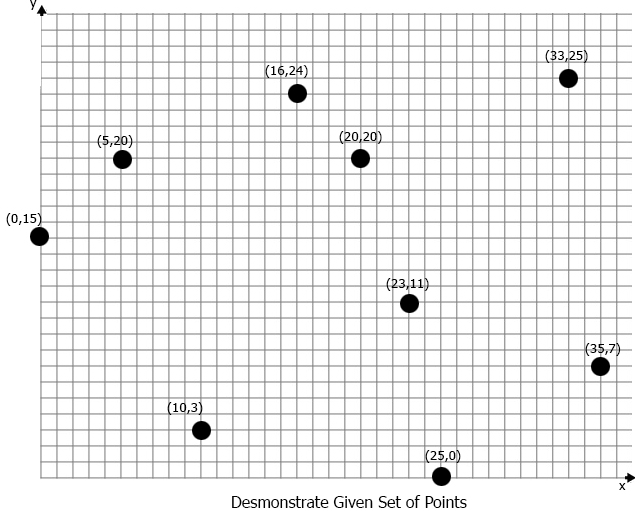
\includegraphics[width=0.7\textwidth]{Brennans1}
	\label{BrennansStuff1}
\end{figure}
\end{frame}

\begin{frame}
\frametitle{Manual MRST Construction via Hanan Grid}
\onslide<1-> \begin{figure}[Hp!]
	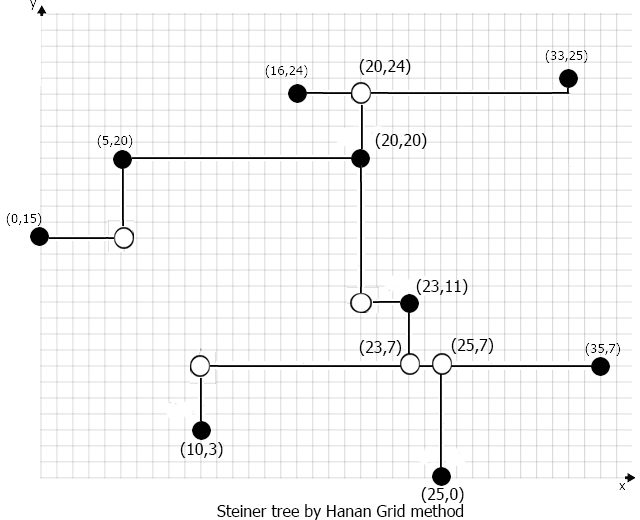
\includegraphics[width=0.7\textwidth]{Brennans2}
	\label{BrennansStuff2}
\end{figure}
\end{frame}

\subsection{Prim's MST Algorithm}
\begin{frame}
\frametitle{Prim's Algorithm}
Generates the minimum spanning tree of a connected graph.
\begin{block}<2->{Algorithm}
\begin{itemize}
\item<2-> {
	Step 1: Create a new tree, adding an arbitrary vertex from the graph.
}
\item<3-> {
	Step 2: Of all edges that connect this tree to vertices not yet in the tree, find the 
	smallest-weight edge and add that to the tree.
}
\item<4-> {
	Step 3: Repeat step 2 until all vertices are in the tree.
}
\end{itemize}
\end{block}
\end{frame}

\section{Solution Methods}

\subsection{(Na\"{i}ve) Hanan/Prim Hybridization}
\begin{frame}
\frametitle{Using MSTs to Find the Minimum Steiner Tree}
\begin{block}{(Na\"{i}ve) Hanan/Prim Hybridization}
\begin{itemize}
\item<1-> {
	Step 1: Construct the Hanan Grid for the given points.
}
\item<2-> {
	Step 2: Repeated remove all 1- and 2-order points not adjacent to a starting vertex.
	
	\onslide<3->(This reduces the Hanan Grid by removing "outside" points.)
}
\item<4-> {
	Step 3: Using Prim's Algorithm, find the MST of this resulting graph. 
}
\end{itemize}
\end{block}
\end{frame}

\subsection{(Smarter) Modifying Prim's Algorithm}
\begin{frame}
\frametitle{Using MSTs to Find the Minimum Steiner Tree}
\begin{block}<1->{(Smarter) Modifying Prim's Algorithm}
\onslide<1-> {Rather than construct a full Hanan Grid, we can apply Prim's algorithm directly; with a few
changes:}
\begin{itemize}
\item<2-> {
In step 2: Keep a running list of distances from each disconnected vertex to its
closest neighbor in the growing tree.

\onslide<2-> {(Needed for variable cardinality of the growing tree.)}
}
\item<3-> {
In step 2: When adding the edge, augment the growing tree with a Steiner point, if needed.

	\begin{itemize}
	\item<4-> {If near an existing path, insert Steiner point on that path.}
	\item<5-> {Otherwise, choose the more "central" Steiner point.}
	\end{itemize}
}
\end{itemize}
\end{block}
\end{frame}

\section{Results \& Discussion}

\subsection{Hanan/Prim Hybridization}
\begin{frame}
\frametitle{Results: Hanan/Prim Hybridization}
 \begin{figure}[htbp!]
 	\vspace{-5pt}
 	\centering
	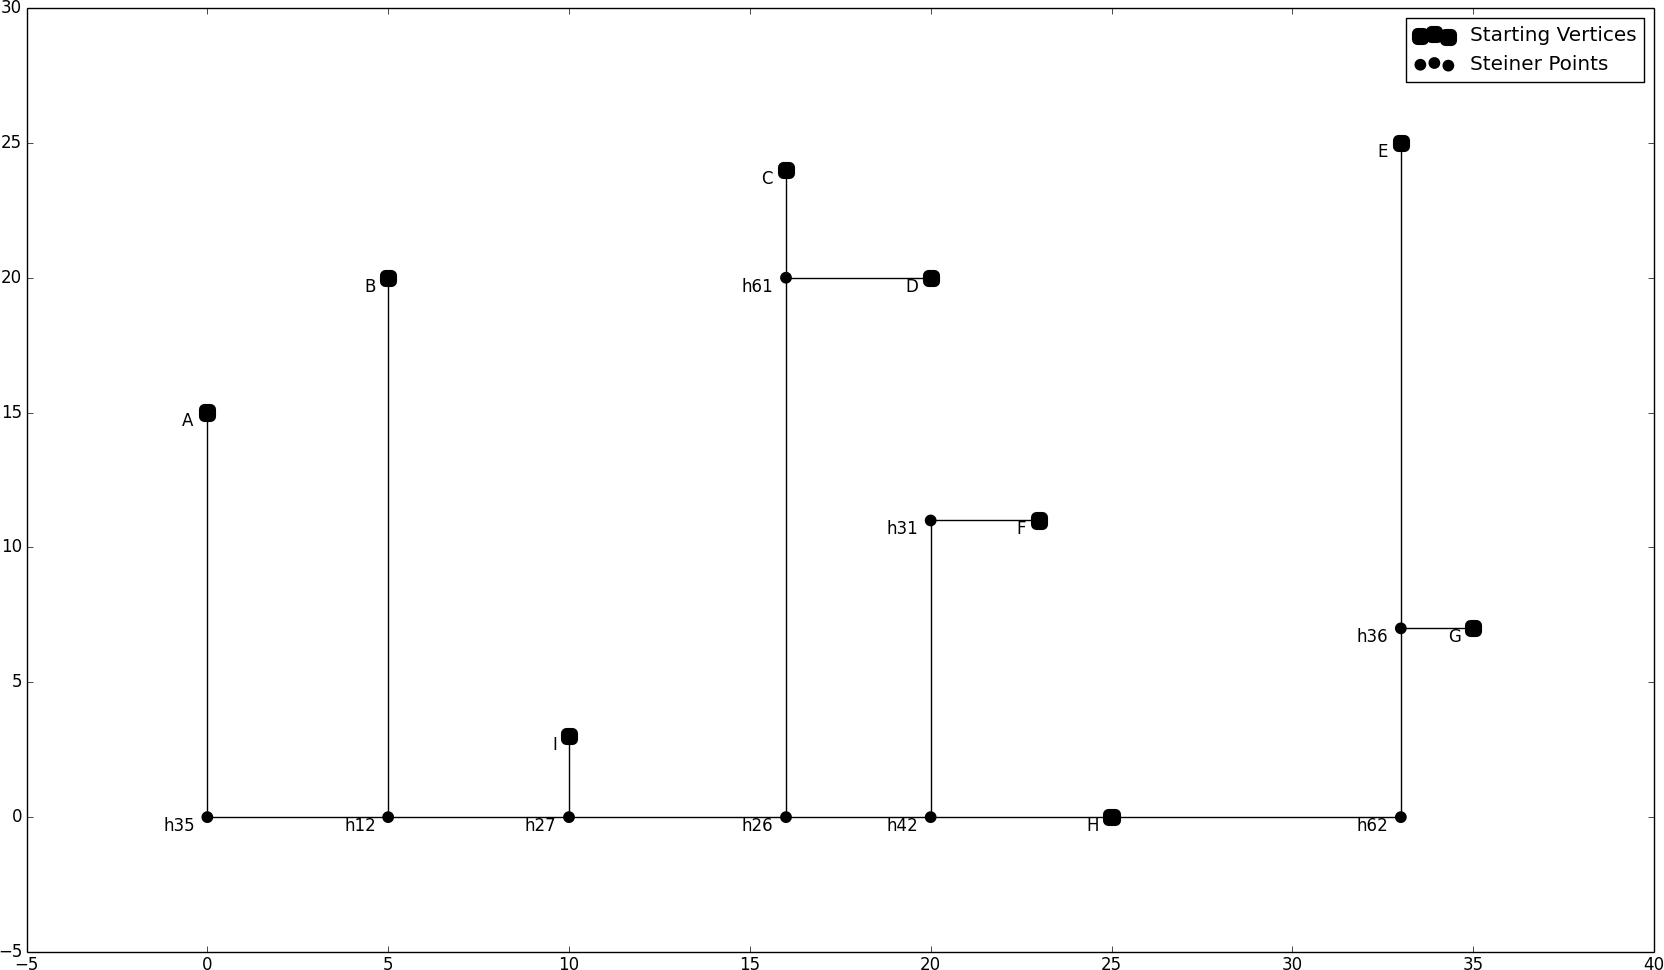
\includegraphics[width=0.95\textwidth]{NaiveResult}
	\caption{Result MRST -- Total Weight: 140 \& 187.59} 
	\label{naiveresult_image}
\end{figure}
\end{frame}

\subsection{Modified Prim's Algorithm}
\begin{frame}
\frametitle{Results: Modified Prim's Algorithm}
 \begin{figure}[htbp!]
 	\vspace{-5pt}
 	\centering
	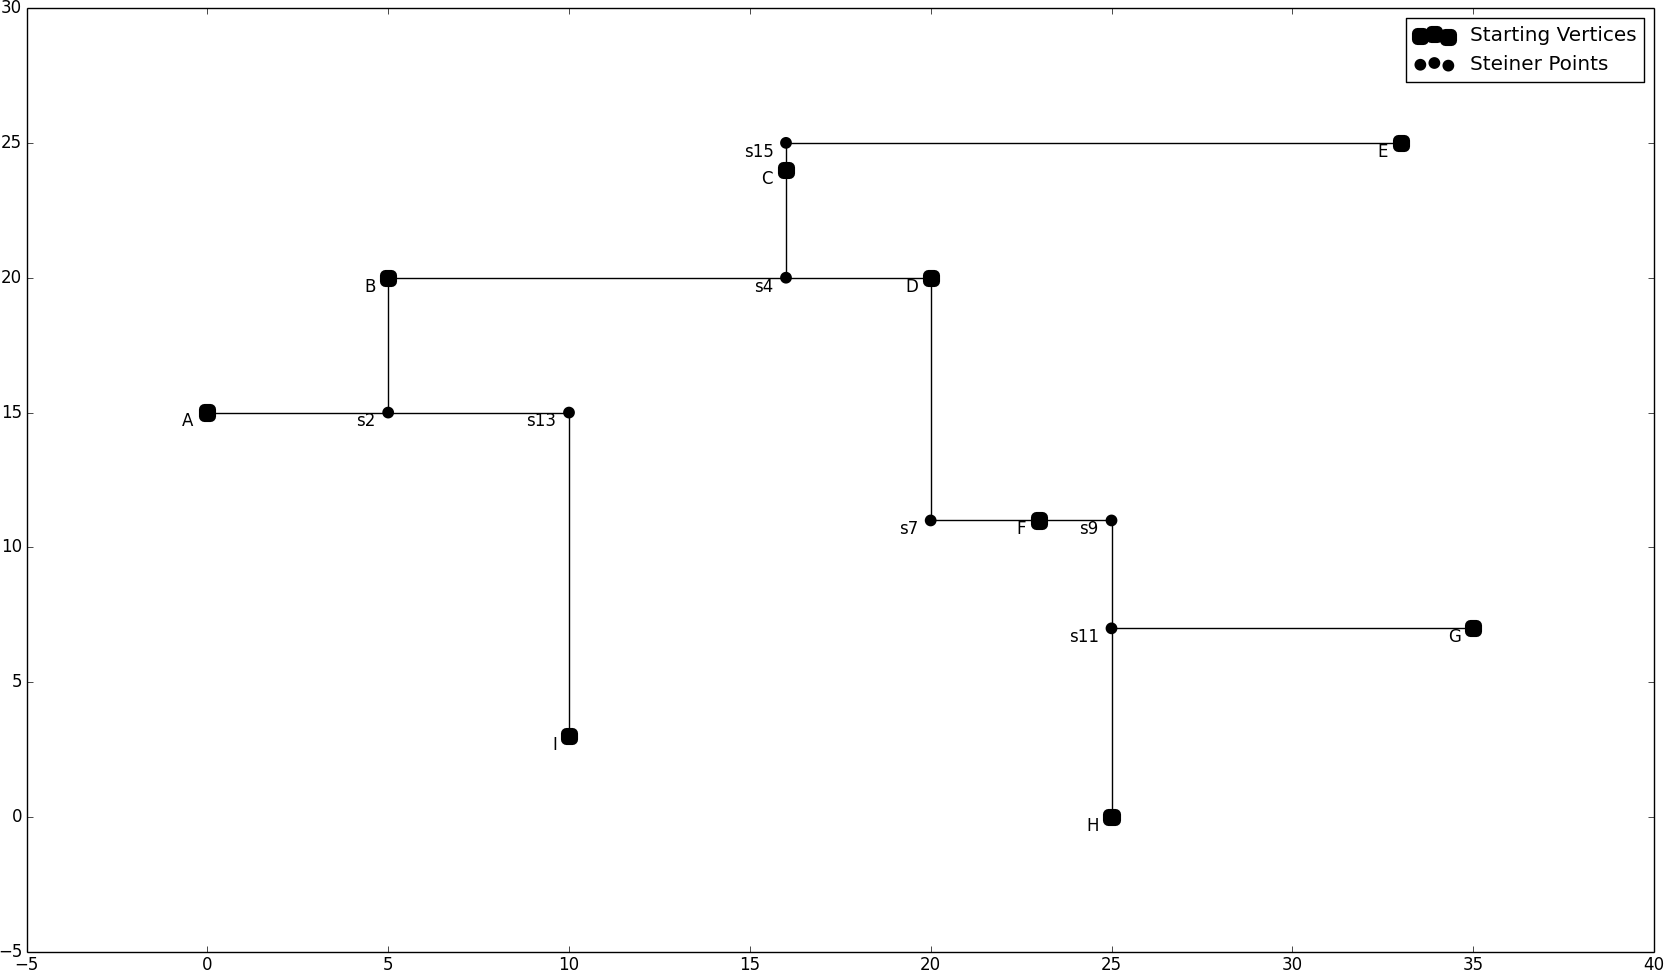
\includegraphics[width=0.95\textwidth]{SmarterResult}
	\caption{Result MRST -- Total Weight: 140 \& 187.59} 
	\label{naiveresult_image}
\end{figure}
\end{frame}

\subsection{Comparison of Methods}
\begin{frame}
\frametitle{Discussion: Comparison of Methods}
\begin{block}<1->{Na\"{i}ve Hanan/Prim Hybridization}
\scriptsize\begin{itemize}
\item<2-> {	 (+) Simpler code! }
\item<3-> {  (+) Holistic algorithm: MRST constructed with full knowledge of graph }
\item<4-> { (--) Constructs entire Hanan Grid: \textbf{very \em{slow}} for large data sets!  \\
e.g.: Several minutes running time for  \(n \approx 50\), hours for \(n \gtrapprox 200\) }
\item<5-> { (--) Likely to use more Steiner points for larger sets. } 
\end{itemize}
\end{block}
\begin{block}<1->{Modified Prim's Algorithm}
\scriptsize\begin{itemize}
\item<2-> {(--) More code complexity (needs to maintain state, e.g. minimum-distance list)} 
\item<3-> {(--) Greedy algorithm: MRST constructed by taking the best choice at each iteration}
\item<4-> { (+) Only adds Steiner points on an as-needed basis: \textbf{much \em{faster}} \\
e.g.: \(< 1\) second  for  \(n \approx 50\), minutes for \(n \gtrapprox 1000\) }
\item<5-> { (+) Attempts to minimize the number of Steiner points to add. }
\end{itemize}
\end{block}
\end{frame}

\subsection{Assumptions \& Flaws}
\begin{frame}
\frametitle{Model Assumptions}
\begin{itemize}
\item<1-> { No obstacles in laying cables (such as gas mains, water pipes, terrain); }
\item<2-> { Cables have uniform cost (i.e., copper coaxial, some fiber optic, etc.) }
\item<3-> { Cables can only go in straight horizontal/vertical lines.
(i.e., Steiner point not necessary only to change direction) }
\end{itemize}
\end{frame}	

\section{Conclusion}

\subsection{Works Cited}
\begin{frame}
\frametitle{Works Cited}
\begin{itemize}
\item {
Dreyer, D., and Overton, M. (1998). \textit{Two heuristics for the Euclidean Steiner tree problem}. Journal of Global Optimization, 13(1), 
95-106.}

\item {
Greenbaum, A. (2006). Discrete Mathematical Model [Lecture Note]. Retrieved from \url{https://www.math.washington.edu/greenbau/Math_381/notes/381notes.pdf}
}

\item {
Hanan, M., \textit{On Steiner's problem with rectilinear distance}. SIAM J. Applied Math., 14:255 -- 265, 1966.
}

\item {
Image: Hanan grid generated for a 5-terminal case. (C) 2007 Jeffrey Sharkey, retrieved from
\url{https://en.wikipedia.org/wiki/File:Hanan5.svg}; licensed under the Creative Commons Attribution-ShareAlike license.
}

\end{itemize}
\end{frame}

\subsection{Thank You}
\begin{frame}
\Huge{\centerline{Thank You}}
\hfill\newline
\centerline{Questions?}
\end{frame}
\end{document} 
